\documentclass{tufte-handout}

\title{Cryptographic Primitives: Hash Functions }

\author[Packer]{Packer Collegiate Institute\\Dr. Anthony Schultz}

%\date{28 March 2010} % without \date command, current date is supplied

%\geometry{showframe} % display margins for debugging page layout

\usepackage{graphicx} % allow embedded images
  \setkeys{Gin}{width=\linewidth,totalheight=\textheight,keepaspectratio}
  \graphicspath{{graphics/}} % set of paths to search for images
\usepackage{amsmath}  % extended mathematics
\usepackage{booktabs} % book-quality tables
\usepackage{units}    % non-stacked fractions and better unit spacing
\usepackage{multicol} % multiple column layout facilities
\usepackage{lipsum}   % filler text
\usepackage{fancyvrb} % extended verbatim environments
  \fvset{fontsize=\normalsize}% default font size for fancy-verbatim environments
  \usepackage{mathtools}
  
  
    %MADNESS
  
  \usepackage[T1]{fontenc} % Use 8-bit encoding that has 256 glyphs
\usepackage{fourier} % Use the Adobe Utopia font for the document - comment this line to return to the LaTeX default
\usepackage[english]{babel} % English language/hyphenation
\usepackage{amsmath,amsfonts,amsthm} % Math packages
\usepackage{mathtools}% http://ctan.org/pkg/mathtools
\usepackage{etoolbox}% http://ctan.org/pkg/etoolbox
\usepackage{lipsum} % Used for inserting dummy 'Lorem ipsum' text into the template
\usepackage{units}% To use \nicefrac
\usepackage{cancel}% To use \cancel
%\usepackage{physymb}%To use r
\usepackage{sectsty} % Allows customizing section commands
\usepackage[dvipsnames]{xcolor}
\usepackage{pgf,tikz}%To draw 
\usepackage{pgfplots}%To draw 
\usetikzlibrary{shapes,arrows}%To draw 
\usetikzlibrary{patterns,fadings}
 \usetikzlibrary{decorations.pathreplacing}%To draw curly braces 
 \usetikzlibrary{snakes}%To draw 
 \usetikzlibrary{spy}%To do zoom-in
 \usepackage{setspace}%Set margins and such
 %\usepackage{3dplot}%To draw in 3D
\usepackage{framed}%To get shade behind text


\definecolor{shadecolor}{rgb}{0.9,0.9,0.9}%setting shade color
\allsectionsfont{\centering \normalfont\scshape} % Make all sections centered, the default font and small caps
  
  

  
  

% Standardize command font styles and environments
\newcommand{\doccmd}[1]{\texttt{\textbackslash#1}}% command name -- adds backslash automatically
\newcommand{\docopt}[1]{\ensuremath{\langle}\textrm{\textit{#1}}\ensuremath{\rangle}}% optional command argument
\newcommand{\docarg}[1]{\textrm{\textit{#1}}}% (required) command argument
\newcommand{\docenv}[1]{\textsf{#1}}% environment name
\newcommand{\docpkg}[1]{\texttt{#1}}% package name
\newcommand{\doccls}[1]{\texttt{#1}}% document class name
\newcommand{\docclsopt}[1]{\texttt{#1}}% document class option name
\newenvironment{docspec}{\begin{quote}\noindent}{\end{quote}}% command specification environment

\begin{document}

\maketitle% this prints the handout title, author, and date
\marginnote[-80pt]{Project folder available at: \\ \href{url}{https://github.com/Trismeg/Packer}}
\begin{marginfigure}[-50pt]%
  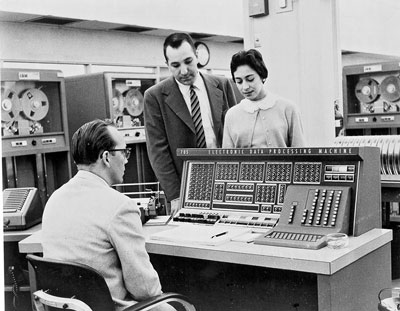
\includegraphics[width=\linewidth]{IBM.jpg}
  \caption{Computer scientists hashing }
  \label{fig:marginfig}
\end{marginfigure}
\begin{abstract}
\noindent
This is an introduction to hash functions.  Hash functions are awesome because they are cryptic and abstract.  They are also great because they are useful and help make the internet run properly.   We will learn the following: 
\begin{itemize}
\item what is a hash function and what are its properties
\item how to use the SHA-256 hash function in Python and from shell
 \item applications of hash functions including cryptographic verification, \\proof of work and proof of existence
 \end{itemize} \end{abstract}

\normalsize

%this generates 1cm of vertical space

\section{Hashing}

\marginnote[-40pt]{
The word \textbf{hash} entered English in the mid 1600's, during the dawn of science.  It meant \textit{to chop into small pieces} and represented a brilliant culinary advancement.  It came from the French \textbf{\textit{hacher}}, \textit{chop up}.  This deriving from Old French \textbf{\textit{hache}}, \textit{ax}.}

\begin{marginfigure}[20 pt]%
  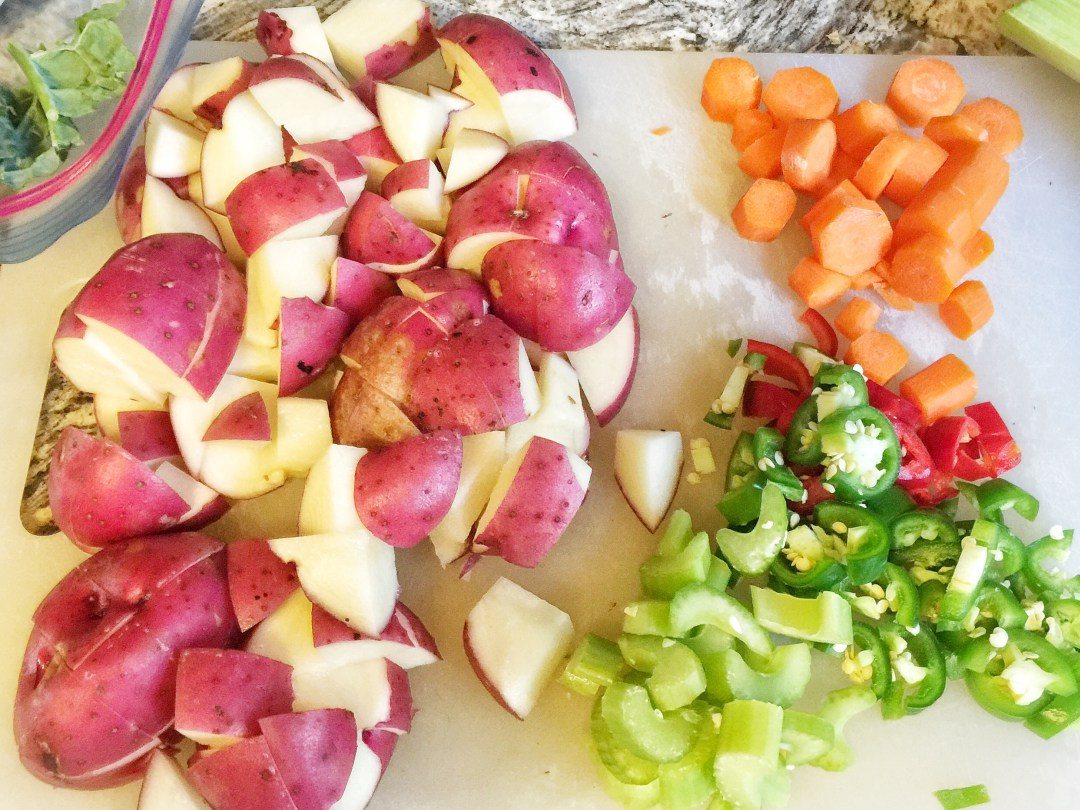
\includegraphics[width=\linewidth]{hash.jpg}
  \caption{Breakfast hash }
  \label{fig:marginfig}
\end{marginfigure}


Hashing is the systematic process of adding entropy to an object in a repeatable but irreversible way.  A cryptographic hash function works like the culinary technique.  It chops up numbers, any data, into a random scramble.  The process is computationally irreversible but fully deterministic and repeatable.  \\

\marginnote[30pt]{A good hash function is a method of randomizing numbers so that no two inputs ever produce the same output.  That is a collision.  It is bad.  Very bad.}
A hash function maps a number $X$ to another number $Y$.
$$\text{Hash}(X)\longrightarrow Y$$
There is no reverse mapping or "un-hashing."  
$$X\mathrlap{\longleftarrow}{\ \ \Large \times}\ \  \text{Hash}^{-1}(Y)$$
A hash function is a non-invertible function.

\section{SHA2}
SHA-2 (Secure Hash Algorithm 2) is a set of cryptographic hash functions designed by the NSA. SHA stands for Secure Hash Algorithm. SHA-256 and SHA-512 are novel hash functions computed with 32-bit and 64-bit words, respectively. They use different shift amounts and additive constants, but their structures are otherwise virtually identical, differing only in the number of rounds.

The SHA-2 hash function is implemented in some widely used security applications and protocols, including TLS and SSL, PGP, SSH, S/MIME, and IPsec.

SHA-256 returns a 64 digit, base 16 number.   The SHA-256 hash of the string "SHA-2 Electric Boogaloo" returns the following:\\
\vspace{0.5cm}
\noindent6f1dceb60c1e2251379c78059a07ec98d6ac368ee2f115c020d753158b16617c

\begin{marginfigure}[-110 pt]%
  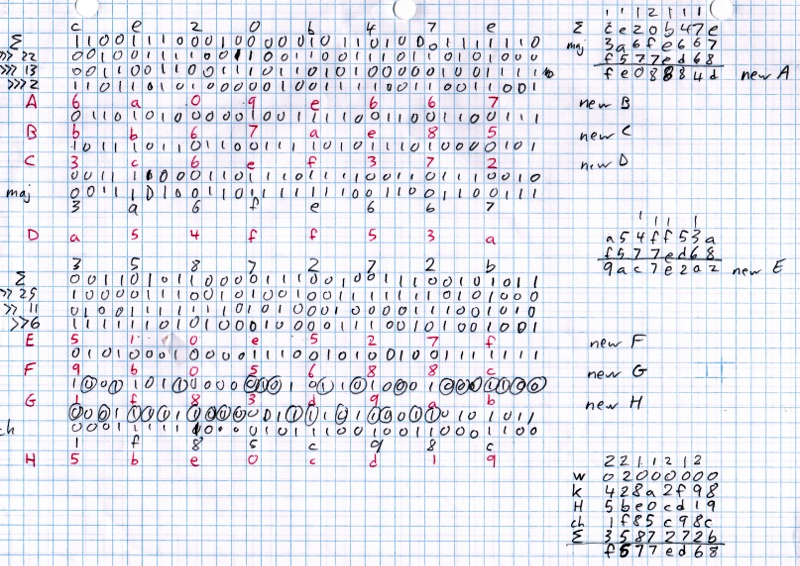
\includegraphics[width=\linewidth]{sha.jpg}
  \caption{SHA-256 by hand}
  \label{fig:marginfig}
\end{marginfigure}

\section{Hashing in Python}
\marginnote[20pt]{Hexidecimal or hex numbers are base 16.  The numerals are written:
$$\texttt{01234567890abdef}$$}
At the command line type the following to get a python shell open.
\small
\begin{shaded}
\begin{verbatim}
$ python
\end{verbatim}
\end{shaded}
\normalsize
Once the python shell is open import the hash library and hash a test message.
\marginnote[-20pt]{The SHA-256 output is 64 digits.  Since the output is hex there are $16^{64}$ possible numbers.  This is on the order of the number of atoms in the whole universe.}
\small
\begin{shaded}
\begin{verbatim}
>>> import hashlib
>>> hashlib.sha256("testing").hexdigest()
'cf80cd8aed482d5d1527d7dc72fceff84e6326592848447d2dc0b0e87dfc9a90'
>>> hashlib.sha256("testing1").hexdigest()
'3e3d6a28351293395ba3a345e79593de3780723a42321204c54b7da49bf3da45'
\end{verbatim}
\end{shaded}
\marginnote[-60pt]{Note that the hash of "testing" and "testing1" is completely different despite the small difference of the input.  This quality is known as entropy.}
\normalsize
This code shows how to hash a file.  This particular program, named "hasher.py" hashes itself.
\small
\begin{framed}
\begin{verbatim}
import hashlib

hasher = hashlib.sha256()
with open("hasher.py", 'rb') as afile:
    buf = afile.read()
    hasher.update(buf)
print(" the hash is ")
print(hasher.hexdigest())
\end{verbatim}
\end{framed}


\marginnote[-120pt]{\\ \ \\ \normalsize
To create this file:\\
\noindent\texttt{\$ touch hasher.py}\\
\noindent\texttt{\$ nano hasher.py}\\
\noindent \textbf{Copy/Paste CTRL+X}\\
\noindent\texttt{\$ python hasher.py}
}
\normalsize
It will output the following.
\small
\begin{shaded}
\begin{verbatim}
 the hash is 
a37d71db6c43c3650ade82ccac7107bad8c268a9b94d03e36d6895eb2edbdd99
\end{verbatim}
\end{shaded}

\begin{marginfigure}%

 $$ 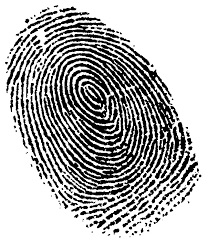
\includegraphics[width=.6\linewidth]{fingerprint.jpg}$$
  \caption{A hash of file is like a digital fingerprint.  It functions as a unique identifier. }
  \label{fig:marginfig}
\end{marginfigure}
\Large
\vspace{2cm}

\textbf{\textit{CHALLENGE!!!!!
\\ Find a number whose hash begins with "87". }}



\newpage
\section{Applications}

\marginnote[15pt]{
\textbf{Verification}\\
\noindent Note the hash code that comes up to verify the software version when you type "python" in the command line.\\ \ \\
\texttt{\$ python}\\
\texttt{Python 2.7.6 v2.7.6:3a1db0d2747e }}

\marginnote[15pt]{
\textbf{Proof of Work}\\
\noindent Hashing requires computing and computing requires energy.  The most efficient computing machinery for the executing SHA-256 is the 16nm BitFury ASIC.  It runs at an efficiency of 0.1 J/GH.}

\marginnote[15pt]{
\textbf{Mining}\\
\noindent The process of Bitcoin mining takes bitcoin transaction data and hashes it.   The miner who discovers a hash with a sufficient number of leading zeros wins a bitcoin prize.  The set of transactions that are hashed together constitute a block.  The transactions are hashed with the previous prize-winning hash and a random number called a "nonce."  The inclusion of the previous block hash order the blocks in time as a sort of chain.  This data structure is called a blockchain.}

\marginnote[15pt]{
\textbf{Digital Fingerprinting}\\
\noindent Since a hash can be used to uniquely identify a file it can be useful as a document reference.  When I write student evaluations every semester I include the SHA-256 hash of their major research papers.  Git, the open source version control system, also uses hashes to uniquely identify every change to a project over time.}

\begin{description}
\item[Verification] SHA-256 is used as part of the process of authenticating Debian GNU/Linux software packages.  If we are downloading software by torrent or loading a page from the internet we can check if the downloaded files are the intended downloads by checking a listed hash for the file.
\item[Partial Knowledge Systems] Unix and Linux vendors are moving to using 256- and 512-bit SHA-2 for secure password hashing.  When storing user login information it is prudent security practice not to directly store passwords but rather hashes of passwords.  If the database is compromised the information will not allow accounts to be compromised.
\item[Proof of Work] Hashing requires computation and this takes energy.  A solution to a hashing challenge shows a cryptographic proof of work.
\item[Proof of Existence] A hash of a file may be encoded in a time-stamped public record in order to document the existence of the file at a specific time.  
\end{description}



\section{Proof of Work Spam Filter}
\marginnote[70pt]{\\ \ \\ \normalsize
To create this file:\\
\noindent\texttt{\$ touch email.py}\\
\noindent\texttt{\$ nano email.py}\\
\noindent \textbf{Copy/Paste CTRL+X}\\
\noindent\texttt{\$ python email.py}
}
\footnotesize
\begin{framed}
\begin{verbatim}
import hashlib

text="Hash this"
recipient="schultz@packer.edu"
nonce=0
state=True

num=3
lead=""
for i in range(num):
    lead=lead+"0"

while state:
    message=recipient+" "+text+" "+str(nonce)
    hashe=hashlib.sha256(message).hexdigest()
    if hashe[0:num]==lead:
        state = False
    else:
        nonce=nonce+1

print "The proper nonce is " + str(nonce)
print message
print hashe
\end{verbatim}
\end{framed}

\normalsize

\begin{marginfigure}%
 $$ 
\includegraphics[width=\linewidth]{hashcash.jpeg}$$
  \caption{Hashing = Energy = Money }
  \label{fig:marginfig}
\end{marginfigure}

Imagine we want to develop an email protocol that will block spam.  One solution to this problem is only to accept email messages which show work.  Spammers send out millions of messages at a time because they can.  If sending an email required some computational work the cost would make it prohibitive for spammers to send out millions of spam emails.  \\
The above code implements such a protocol.  Imagine only message whose hash has a sufficient number of leading zeros are accepted by the recipient server.  In the code the variable \texttt{num} determines the number of leading zeros required.  Notice the higher this number the longer it takes to generate an acceptable method.  The nonce value allow the sender to change the hash output without changing the recipient or message content. \footnote{This type of proof-of-work email system was proposed in May 1997 by Adam Back under the name Hashcash.}

\section{Proof of Existence of Our Spam Filter}
Imagine that we want to protect our intellectual property for our spam fighting email system.  We hay take the hash of 

\small
\begin{framed}
\begin{verbatim}
import hashlib

hasher = hashlib.sha256()
with open("email.py", 'rb') as afile:
    buf = afile.read()
    hasher.update(buf)
print(" the hash is ")
print(hasher.hexdigest())
\end{verbatim}
\end{framed}

\marginnote[-80pt]{We may also achieve this using the following shell command.\\ \ \\
\texttt{\$ shasum -a 256 email.py}}

\normalsize
It will output the following:
\small
\begin{shaded}
\begin{verbatim}
 the hash is 
217c72a2b3a355bec2bda20e5280eaabae8fb445f8cf01666cd213fee7be2cde
\end{verbatim}
\end{shaded}

\marginnote[-40pt]{Many services provide the ability to hash a document and record the resulting hash in the blockchain.  It is a notary service.  One such service started by Manuel Araoz:\\
\href{url}{https://www.proofofexistence.com}}
\marginnote[30pt]{Inclusion of a hash in a blockchain constitutes legal proof of existence in the state of Vermont.\\ \href{url}{http://goo.gl/ZpzPjv}}


\normalsize
As a unique identifier for the file "email.py" the hash may be used as a proof of existence for the file without revealing the file itself.  All that is required is a trusted timestamp.  We could seal this in an envelope and mail it to ourselves.  The postmark can serve as a timestamp.  Another option is that we could take out an add in the New York Times, our trusted paper of record.  The recording of the hash in the paper can be proof at a later date that the hash existed and thus the file existed.\\
Another interesting solution is to take the hash value and encode it in a transaction in a blockchain.  This has been done for this file.\footnote{\href{url}{https://goo.gl/ULQwKD}}



%\bibliography{sample-handout}
%\bibliographystyle{plainnat}



\end{document}
